\documentclass[twoside]{book}

% Packages required by doxygen
\usepackage{fixltx2e}
\usepackage{calc}
\usepackage{doxygen}
\usepackage[export]{adjustbox} % also loads graphicx
\usepackage{graphicx}
\usepackage[utf8]{inputenc}
\usepackage{makeidx}
\usepackage{multicol}
\usepackage{multirow}
\PassOptionsToPackage{warn}{textcomp}
\usepackage{textcomp}
\usepackage[nointegrals]{wasysym}
\usepackage[table]{xcolor}

% Font selection
\usepackage[T1]{fontenc}
\usepackage[scaled=.90]{helvet}
\usepackage{courier}
\usepackage{amssymb}
\usepackage{sectsty}
\renewcommand{\familydefault}{\sfdefault}
\allsectionsfont{%
  \fontseries{bc}\selectfont%
  \color{darkgray}%
}
\renewcommand{\DoxyLabelFont}{%
  \fontseries{bc}\selectfont%
  \color{darkgray}%
}
\newcommand{\+}{\discretionary{\mbox{\scriptsize$\hookleftarrow$}}{}{}}

% Page & text layout
\usepackage{geometry}
\geometry{%
  a4paper,%
  top=2.5cm,%
  bottom=2.5cm,%
  left=2.5cm,%
  right=2.5cm%
}
\tolerance=750
\hfuzz=15pt
\hbadness=750
\setlength{\emergencystretch}{15pt}
\setlength{\parindent}{0cm}
\setlength{\parskip}{3ex plus 2ex minus 2ex}
\makeatletter
\renewcommand{\paragraph}{%
  \@startsection{paragraph}{4}{0ex}{-1.0ex}{1.0ex}{%
    \normalfont\normalsize\bfseries\SS@parafont%
  }%
}
\renewcommand{\subparagraph}{%
  \@startsection{subparagraph}{5}{0ex}{-1.0ex}{1.0ex}{%
    \normalfont\normalsize\bfseries\SS@subparafont%
  }%
}
\makeatother

% Headers & footers
\usepackage{fancyhdr}
\pagestyle{fancyplain}
\fancyhead[LE]{\fancyplain{}{\bfseries\thepage}}
\fancyhead[CE]{\fancyplain{}{}}
\fancyhead[RE]{\fancyplain{}{\bfseries\leftmark}}
\fancyhead[LO]{\fancyplain{}{\bfseries\rightmark}}
\fancyhead[CO]{\fancyplain{}{}}
\fancyhead[RO]{\fancyplain{}{\bfseries\thepage}}
\fancyfoot[LE]{\fancyplain{}{}}
\fancyfoot[CE]{\fancyplain{}{}}
\fancyfoot[RE]{\fancyplain{}{\bfseries\scriptsize Generated by Doxygen }}
\fancyfoot[LO]{\fancyplain{}{\bfseries\scriptsize Generated by Doxygen }}
\fancyfoot[CO]{\fancyplain{}{}}
\fancyfoot[RO]{\fancyplain{}{}}
\renewcommand{\footrulewidth}{0.4pt}
\renewcommand{\chaptermark}[1]{%
  \markboth{#1}{}%
}
\renewcommand{\sectionmark}[1]{%
  \markright{\thesection\ #1}%
}

% Indices & bibliography
\usepackage{natbib}
\usepackage[titles]{tocloft}
\setcounter{tocdepth}{3}
\setcounter{secnumdepth}{5}
\makeindex

% Hyperlinks (required, but should be loaded last)
\usepackage{ifpdf}
\ifpdf
  \usepackage[pdftex,pagebackref=true]{hyperref}
\else
  \usepackage[ps2pdf,pagebackref=true]{hyperref}
\fi
\hypersetup{%
  colorlinks=true,%
  linkcolor=blue,%
  citecolor=blue,%
  unicode%
}

% Custom commands
\newcommand{\clearemptydoublepage}{%
  \newpage{\pagestyle{empty}\cleardoublepage}%
}

\usepackage{caption}
\captionsetup{labelsep=space,justification=centering,font={bf},singlelinecheck=off,skip=4pt,position=top}

%===== C O N T E N T S =====

\begin{document}

% Titlepage & ToC
\hypersetup{pageanchor=false,
             bookmarksnumbered=true,
             pdfencoding=unicode
            }
\pagenumbering{alph}
\begin{titlepage}
\vspace*{7cm}
\begin{center}%
{\Large Tic\+Tac\+Toe \\[1ex]\large 1.\+0 }\\
\vspace*{1cm}
{\large Generated by Doxygen 1.8.13}\\
\end{center}
\end{titlepage}
\clearemptydoublepage
\pagenumbering{roman}
\tableofcontents
\clearemptydoublepage
\pagenumbering{arabic}
\hypersetup{pageanchor=true}

%--- Begin generated contents ---
\chapter{Hierarchical Index}
\section{Class Hierarchy}
This inheritance list is sorted roughly, but not completely, alphabetically\+:\begin{DoxyCompactList}
\item \contentsline{section}{Tic\+Tac\+Toe}{\pageref{class_tic_tac_toe}}{}
\item \contentsline{section}{Tic\+Tac\+Toe\+Abstract\+Player}{\pageref{class_tic_tac_toe_abstract_player}}{}
\begin{DoxyCompactList}
\item \contentsline{section}{Tic\+Tac\+Toe\+Bot}{\pageref{class_tic_tac_toe_bot}}{}
\end{DoxyCompactList}
\end{DoxyCompactList}

\chapter{Class Index}
\section{Class List}
Here are the classes, structs, unions and interfaces with brief descriptions\+:\begin{DoxyCompactList}
\item\contentsline{section}{\hyperlink{class_tic_tac_toe}{Tic\+Tac\+Toe} }{\pageref{class_tic_tac_toe}}{}
\item\contentsline{section}{\hyperlink{class_tic_tac_toe_abstract_player}{Tic\+Tac\+Toe\+Abstract\+Player} }{\pageref{class_tic_tac_toe_abstract_player}}{}
\item\contentsline{section}{\hyperlink{class_tic_tac_toe_bot}{Tic\+Tac\+Toe\+Bot} }{\pageref{class_tic_tac_toe_bot}}{}
\end{DoxyCompactList}

\chapter{File Index}
\section{File List}
Here is a list of all files with brief descriptions\+:\begin{DoxyCompactList}
\item\contentsline{section}{\hyperlink{common__defs_8h}{common\+\_\+defs.\+h} }{\pageref{common__defs_8h}}{}
\item\contentsline{section}{\hyperlink{main_8cpp}{main.\+cpp} }{\pageref{main_8cpp}}{}
\item\contentsline{section}{\hyperlink{tictactoe_8cpp}{tictactoe.\+cpp} }{\pageref{tictactoe_8cpp}}{}
\item\contentsline{section}{\hyperlink{tictactoe_8h}{tictactoe.\+h} }{\pageref{tictactoe_8h}}{}
\item\contentsline{section}{\hyperlink{tictactoeabstractplayer_8cpp}{tictactoeabstractplayer.\+cpp} }{\pageref{tictactoeabstractplayer_8cpp}}{}
\item\contentsline{section}{\hyperlink{tictactoeabstractplayer_8h}{tictactoeabstractplayer.\+h} }{\pageref{tictactoeabstractplayer_8h}}{}
\item\contentsline{section}{\hyperlink{tictactoebot_8cpp}{tictactoebot.\+cpp} }{\pageref{tictactoebot_8cpp}}{}
\item\contentsline{section}{\hyperlink{tictactoebot_8h}{tictactoebot.\+h} }{\pageref{tictactoebot_8h}}{}
\end{DoxyCompactList}

\chapter{Class Documentation}
\hypertarget{class_tic_tac_toe}{}\section{Tic\+Tac\+Toe Class Reference}
\label{class_tic_tac_toe}\index{Tic\+Tac\+Toe@{Tic\+Tac\+Toe}}


{\ttfamily \#include $<$tictactoe.\+h$>$}

\subsection*{Public Member Functions}
\begin{DoxyCompactItemize}
\item 
\hyperlink{class_tic_tac_toe_a27555f19d0f8041ef8ce9a268ec0554c}{Tic\+Tac\+Toe} (size\+\_\+t size)
\item 
\hyperlink{class_tic_tac_toe_a85910bb5d348929c9fef9f0b23813a60}{Tic\+Tac\+Toe} (const \hyperlink{common__defs_8h_a0dc5e1c0d1c3d4b1e210c805de5ca27b}{Board} \&board, \hyperlink{common__defs_8h_a9c8780378078e51e7c9041cbac392db9}{Player} player=\hyperlink{common__defs_8h_a9c8780378078e51e7c9041cbac392db9a37a6259cc0c1dae299a7866489dff0bd}{Player\+::null})
\item 
std\+::pair$<$ \hyperlink{common__defs_8h_a9c8780378078e51e7c9041cbac392db9}{Player}, \hyperlink{common__defs_8h_a67a0db04d321a74b7e7fcfd3f1a3f70b}{Status} $>$ \hyperlink{class_tic_tac_toe_a5bbb9eeb1ab08a3d9ce857cecc3d7ffc}{move} (const \hyperlink{common__defs_8h_af9623b96ea87eb8f2d0fe97e45b0f79a}{Position} \&pos, \hyperlink{common__defs_8h_a9c8780378078e51e7c9041cbac392db9}{Player} player=\hyperlink{common__defs_8h_a9c8780378078e51e7c9041cbac392db9a37a6259cc0c1dae299a7866489dff0bd}{Player\+::null})
\begin{DoxyCompactList}\small\item\em move performs player movement \end{DoxyCompactList}\item 
\hyperlink{common__defs_8h_a9c8780378078e51e7c9041cbac392db9}{Player} \hyperlink{class_tic_tac_toe_af58c3728beedc8d250927f1f07c03dee}{active\+\_\+player} () const
\begin{DoxyCompactList}\small\item\em active\+\_\+player geter for active player \end{DoxyCompactList}\item 
const \hyperlink{common__defs_8h_a9c8780378078e51e7c9041cbac392db9}{Player} \& \hyperlink{class_tic_tac_toe_abafc7ee6550f447cf9e4c798a3658ab7}{field} (const size\+\_\+t \&row, const size\+\_\+t \&col) const
\begin{DoxyCompactList}\small\item\em field geter for particular field of the game board \end{DoxyCompactList}\item 
const std\+::vector$<$ std\+::vector$<$ \hyperlink{common__defs_8h_a9c8780378078e51e7c9041cbac392db9}{Player} $>$ $>$ \& \hyperlink{class_tic_tac_toe_a2bd8a25c0a5885b76ac84a201751b307}{state} () const
\begin{DoxyCompactList}\small\item\em state geter for board \end{DoxyCompactList}\item 
void \hyperlink{class_tic_tac_toe_a3b71a1e724f9af69d0fb8ba3dd848942}{debug} () const
\begin{DoxyCompactList}\small\item\em debug prints board to std out \end{DoxyCompactList}\end{DoxyCompactItemize}
\subsection*{Static Public Member Functions}
\begin{DoxyCompactItemize}
\item 
static char \hyperlink{class_tic_tac_toe_a829574b09a8672b4fb65d4a7cfeba83e}{convert} (\hyperlink{common__defs_8h_a9c8780378078e51e7c9041cbac392db9}{Player} p)
\begin{DoxyCompactList}\small\item\em convert converts Player enum to char symbol \end{DoxyCompactList}\end{DoxyCompactItemize}
\subsection*{Protected Member Functions}
\begin{DoxyCompactItemize}
\item 
bool \hyperlink{class_tic_tac_toe_a8495d66a8662f19b33be04e41da9a133}{check\+\_\+move} (size\+\_\+t row, size\+\_\+t col, \hyperlink{common__defs_8h_a9c8780378078e51e7c9041cbac392db9}{Player} player) const
\begin{DoxyCompactList}\small\item\em check\+\_\+move verifies whether the move is possible \end{DoxyCompactList}\item 
\hyperlink{common__defs_8h_a67a0db04d321a74b7e7fcfd3f1a3f70b}{Status} \hyperlink{class_tic_tac_toe_a592cbbdeee049391313a0712ca12589c}{is\+\_\+finished} () const
\begin{DoxyCompactList}\small\item\em is\+\_\+finished virifies whether the game was finished (win or drawn) \end{DoxyCompactList}\end{DoxyCompactItemize}
\subsection*{Protected Attributes}
\begin{DoxyCompactItemize}
\item 
size\+\_\+t \hyperlink{class_tic_tac_toe_afc64aed11c9b53b699c61a8cc3b58dc2}{size\+\_\+}
\item 
\hyperlink{common__defs_8h_a0dc5e1c0d1c3d4b1e210c805de5ca27b}{Board} \hyperlink{class_tic_tac_toe_a577cac99116dca16cfa05890152c2d55}{board\+\_\+}
\item 
\hyperlink{common__defs_8h_a9c8780378078e51e7c9041cbac392db9}{Player} \hyperlink{class_tic_tac_toe_a5acba985df8b3d158783a5f4f3521f2e}{active\+\_\+player\+\_\+}
\end{DoxyCompactItemize}


\subsection{Detailed Description}


Definition at line 7 of file tictactoe.\+h.



\subsection{Constructor \& Destructor Documentation}
\mbox{\Hypertarget{class_tic_tac_toe_a27555f19d0f8041ef8ce9a268ec0554c}\label{class_tic_tac_toe_a27555f19d0f8041ef8ce9a268ec0554c}} 
\index{Tic\+Tac\+Toe@{Tic\+Tac\+Toe}!Tic\+Tac\+Toe@{Tic\+Tac\+Toe}}
\index{Tic\+Tac\+Toe@{Tic\+Tac\+Toe}!Tic\+Tac\+Toe@{Tic\+Tac\+Toe}}
\subsubsection{\texorpdfstring{Tic\+Tac\+Toe()}{TicTacToe()}\hspace{0.1cm}{\footnotesize\ttfamily [1/2]}}
{\footnotesize\ttfamily Tic\+Tac\+Toe\+::\+Tic\+Tac\+Toe (\begin{DoxyParamCaption}\item[{size\+\_\+t}]{size }\end{DoxyParamCaption})}



Definition at line 3 of file tictactoe.\+cpp.

\mbox{\Hypertarget{class_tic_tac_toe_a85910bb5d348929c9fef9f0b23813a60}\label{class_tic_tac_toe_a85910bb5d348929c9fef9f0b23813a60}} 
\index{Tic\+Tac\+Toe@{Tic\+Tac\+Toe}!Tic\+Tac\+Toe@{Tic\+Tac\+Toe}}
\index{Tic\+Tac\+Toe@{Tic\+Tac\+Toe}!Tic\+Tac\+Toe@{Tic\+Tac\+Toe}}
\subsubsection{\texorpdfstring{Tic\+Tac\+Toe()}{TicTacToe()}\hspace{0.1cm}{\footnotesize\ttfamily [2/2]}}
{\footnotesize\ttfamily Tic\+Tac\+Toe\+::\+Tic\+Tac\+Toe (\begin{DoxyParamCaption}\item[{const \hyperlink{common__defs_8h_a0dc5e1c0d1c3d4b1e210c805de5ca27b}{Board} \&}]{board,  }\item[{\hyperlink{common__defs_8h_a9c8780378078e51e7c9041cbac392db9}{Player}}]{player = {\ttfamily \hyperlink{common__defs_8h_a9c8780378078e51e7c9041cbac392db9a37a6259cc0c1dae299a7866489dff0bd}{Player\+::null}} }\end{DoxyParamCaption})}



Definition at line 8 of file tictactoe.\+cpp.



\subsection{Member Function Documentation}
\mbox{\Hypertarget{class_tic_tac_toe_af58c3728beedc8d250927f1f07c03dee}\label{class_tic_tac_toe_af58c3728beedc8d250927f1f07c03dee}} 
\index{Tic\+Tac\+Toe@{Tic\+Tac\+Toe}!active\+\_\+player@{active\+\_\+player}}
\index{active\+\_\+player@{active\+\_\+player}!Tic\+Tac\+Toe@{Tic\+Tac\+Toe}}
\subsubsection{\texorpdfstring{active\+\_\+player()}{active\_player()}}
{\footnotesize\ttfamily \hyperlink{common__defs_8h_a9c8780378078e51e7c9041cbac392db9}{Player} Tic\+Tac\+Toe\+::active\+\_\+player (\begin{DoxyParamCaption}{ }\end{DoxyParamCaption}) const\hspace{0.3cm}{\ttfamily [inline]}}



active\+\_\+player geter for active player 

\begin{DoxyReturn}{Returns}
player id \hyperlink{common__defs_8h_a9c8780378078e51e7c9041cbac392db9a22aadb26447d87b550b155a4d764fad0}{Player\+::cross} or \hyperlink{common__defs_8h_a9c8780378078e51e7c9041cbac392db9a9b6ddeba5b33e577c07c35d8505c6072}{Player\+::circle} 
\end{DoxyReturn}


Definition at line 28 of file tictactoe.\+h.

\mbox{\Hypertarget{class_tic_tac_toe_a8495d66a8662f19b33be04e41da9a133}\label{class_tic_tac_toe_a8495d66a8662f19b33be04e41da9a133}} 
\index{Tic\+Tac\+Toe@{Tic\+Tac\+Toe}!check\+\_\+move@{check\+\_\+move}}
\index{check\+\_\+move@{check\+\_\+move}!Tic\+Tac\+Toe@{Tic\+Tac\+Toe}}
\subsubsection{\texorpdfstring{check\+\_\+move()}{check\_move()}}
{\footnotesize\ttfamily bool Tic\+Tac\+Toe\+::check\+\_\+move (\begin{DoxyParamCaption}\item[{size\+\_\+t}]{row,  }\item[{size\+\_\+t}]{col,  }\item[{\hyperlink{common__defs_8h_a9c8780378078e51e7c9041cbac392db9}{Player}}]{player }\end{DoxyParamCaption}) const\hspace{0.3cm}{\ttfamily [protected]}}



check\+\_\+move verifies whether the move is possible 


\begin{DoxyParams}{Parameters}
{\em row} & row of the board $<$0..size\+\_\+) \\
\hline
{\em col} & column of the board $<$0..size\+\_\+) \\
\hline
{\em player} & player id \\
\hline
\end{DoxyParams}
\begin{DoxyReturn}{Returns}
true -\/ if move is correct, otherwise false 
\end{DoxyReturn}


Definition at line 30 of file tictactoe.\+cpp.

\mbox{\Hypertarget{class_tic_tac_toe_a829574b09a8672b4fb65d4a7cfeba83e}\label{class_tic_tac_toe_a829574b09a8672b4fb65d4a7cfeba83e}} 
\index{Tic\+Tac\+Toe@{Tic\+Tac\+Toe}!convert@{convert}}
\index{convert@{convert}!Tic\+Tac\+Toe@{Tic\+Tac\+Toe}}
\subsubsection{\texorpdfstring{convert()}{convert()}}
{\footnotesize\ttfamily char Tic\+Tac\+Toe\+::convert (\begin{DoxyParamCaption}\item[{\hyperlink{common__defs_8h_a9c8780378078e51e7c9041cbac392db9}{Player}}]{p }\end{DoxyParamCaption})\hspace{0.3cm}{\ttfamily [static]}}



convert converts Player enum to char symbol 


\begin{DoxyParams}{Parameters}
{\em p} & player enum (corss circle or empty) \\
\hline
\end{DoxyParams}
\begin{DoxyReturn}{Returns}
character symbol of the player 
\end{DoxyReturn}


Definition at line 81 of file tictactoe.\+cpp.

\mbox{\Hypertarget{class_tic_tac_toe_a3b71a1e724f9af69d0fb8ba3dd848942}\label{class_tic_tac_toe_a3b71a1e724f9af69d0fb8ba3dd848942}} 
\index{Tic\+Tac\+Toe@{Tic\+Tac\+Toe}!debug@{debug}}
\index{debug@{debug}!Tic\+Tac\+Toe@{Tic\+Tac\+Toe}}
\subsubsection{\texorpdfstring{debug()}{debug()}}
{\footnotesize\ttfamily void Tic\+Tac\+Toe\+::debug (\begin{DoxyParamCaption}{ }\end{DoxyParamCaption}) const}



debug prints board to std out 



Definition at line 91 of file tictactoe.\+cpp.

\mbox{\Hypertarget{class_tic_tac_toe_abafc7ee6550f447cf9e4c798a3658ab7}\label{class_tic_tac_toe_abafc7ee6550f447cf9e4c798a3658ab7}} 
\index{Tic\+Tac\+Toe@{Tic\+Tac\+Toe}!field@{field}}
\index{field@{field}!Tic\+Tac\+Toe@{Tic\+Tac\+Toe}}
\subsubsection{\texorpdfstring{field()}{field()}}
{\footnotesize\ttfamily const \hyperlink{common__defs_8h_a9c8780378078e51e7c9041cbac392db9}{Player}\& Tic\+Tac\+Toe\+::field (\begin{DoxyParamCaption}\item[{const size\+\_\+t \&}]{row,  }\item[{const size\+\_\+t \&}]{col }\end{DoxyParamCaption}) const\hspace{0.3cm}{\ttfamily [inline]}}



field geter for particular field of the game board 


\begin{DoxyParams}{Parameters}
{\em row} & \\
\hline
{\em col} & \\
\hline
\end{DoxyParams}
\begin{DoxyReturn}{Returns}
field state \hyperlink{common__defs_8h_a9c8780378078e51e7c9041cbac392db9a37a6259cc0c1dae299a7866489dff0bd}{Player\+::null} field is empty, \hyperlink{common__defs_8h_a9c8780378078e51e7c9041cbac392db9a22aadb26447d87b550b155a4d764fad0}{Player\+::cross}, \hyperlink{common__defs_8h_a9c8780378078e51e7c9041cbac392db9a9b6ddeba5b33e577c07c35d8505c6072}{Player\+::circle} -\/ represent the player id 
\end{DoxyReturn}


Definition at line 35 of file tictactoe.\+h.

\mbox{\Hypertarget{class_tic_tac_toe_a592cbbdeee049391313a0712ca12589c}\label{class_tic_tac_toe_a592cbbdeee049391313a0712ca12589c}} 
\index{Tic\+Tac\+Toe@{Tic\+Tac\+Toe}!is\+\_\+finished@{is\+\_\+finished}}
\index{is\+\_\+finished@{is\+\_\+finished}!Tic\+Tac\+Toe@{Tic\+Tac\+Toe}}
\subsubsection{\texorpdfstring{is\+\_\+finished()}{is\_finished()}}
{\footnotesize\ttfamily \hyperlink{common__defs_8h_a67a0db04d321a74b7e7fcfd3f1a3f70b}{Status} Tic\+Tac\+Toe\+::is\+\_\+finished (\begin{DoxyParamCaption}{ }\end{DoxyParamCaption}) const\hspace{0.3cm}{\ttfamily [protected]}}



is\+\_\+finished virifies whether the game was finished (win or drawn) 

\begin{DoxyReturn}{Returns}
\hyperlink{common__defs_8h_a67a0db04d321a74b7e7fcfd3f1a3f70ba0b08bd98d279b88859b628cd8c061ae0}{Status\+::win} if active layer won, Status\+::drawn if drawn occured, \hyperlink{common__defs_8h_a67a0db04d321a74b7e7fcfd3f1a3f70ba3734a903022249b3010be1897042568e}{Status\+::move} if the game can be continued 
\end{DoxyReturn}


Definition at line 35 of file tictactoe.\+cpp.

\mbox{\Hypertarget{class_tic_tac_toe_a5bbb9eeb1ab08a3d9ce857cecc3d7ffc}\label{class_tic_tac_toe_a5bbb9eeb1ab08a3d9ce857cecc3d7ffc}} 
\index{Tic\+Tac\+Toe@{Tic\+Tac\+Toe}!move@{move}}
\index{move@{move}!Tic\+Tac\+Toe@{Tic\+Tac\+Toe}}
\subsubsection{\texorpdfstring{move()}{move()}}
{\footnotesize\ttfamily std\+::pair$<$ \hyperlink{common__defs_8h_a9c8780378078e51e7c9041cbac392db9}{Player}, \hyperlink{common__defs_8h_a67a0db04d321a74b7e7fcfd3f1a3f70b}{Status} $>$ Tic\+Tac\+Toe\+::move (\begin{DoxyParamCaption}\item[{const \hyperlink{common__defs_8h_af9623b96ea87eb8f2d0fe97e45b0f79a}{Position} \&}]{pos,  }\item[{\hyperlink{common__defs_8h_a9c8780378078e51e7c9041cbac392db9}{Player}}]{player = {\ttfamily \hyperlink{common__defs_8h_a9c8780378078e51e7c9041cbac392db9a37a6259cc0c1dae299a7866489dff0bd}{Player\+::null}} }\end{DoxyParamCaption})}



move performs player movement 


\begin{DoxyParams}{Parameters}
{\em pos} & std\+::pair representing row and columns of the gameboard $<$0;size\+\_\+) \\
\hline
{\em player} & id of the player performing move \\
\hline
\end{DoxyParams}
\begin{DoxyReturn}{Returns}
std\+::pair consisted of\+: the active player id (if the move was correct the id of the next player, if not the active player is not changed). The Status represents the game state Status\+:move -\/ move is possible, or Status\+:win or Status\+::drawn 
\end{DoxyReturn}


Definition at line 12 of file tictactoe.\+cpp.

\mbox{\Hypertarget{class_tic_tac_toe_a2bd8a25c0a5885b76ac84a201751b307}\label{class_tic_tac_toe_a2bd8a25c0a5885b76ac84a201751b307}} 
\index{Tic\+Tac\+Toe@{Tic\+Tac\+Toe}!state@{state}}
\index{state@{state}!Tic\+Tac\+Toe@{Tic\+Tac\+Toe}}
\subsubsection{\texorpdfstring{state()}{state()}}
{\footnotesize\ttfamily const std\+::vector$<$std\+::vector$<$\hyperlink{common__defs_8h_a9c8780378078e51e7c9041cbac392db9}{Player}$>$ $>$\& Tic\+Tac\+Toe\+::state (\begin{DoxyParamCaption}{ }\end{DoxyParamCaption}) const\hspace{0.3cm}{\ttfamily [inline]}}



state geter for board 

\begin{DoxyReturn}{Returns}
2d std\+::vector representing board 
\end{DoxyReturn}


Definition at line 41 of file tictactoe.\+h.



\subsection{Member Data Documentation}
\mbox{\Hypertarget{class_tic_tac_toe_a5acba985df8b3d158783a5f4f3521f2e}\label{class_tic_tac_toe_a5acba985df8b3d158783a5f4f3521f2e}} 
\index{Tic\+Tac\+Toe@{Tic\+Tac\+Toe}!active\+\_\+player\+\_\+@{active\+\_\+player\+\_\+}}
\index{active\+\_\+player\+\_\+@{active\+\_\+player\+\_\+}!Tic\+Tac\+Toe@{Tic\+Tac\+Toe}}
\subsubsection{\texorpdfstring{active\+\_\+player\+\_\+}{active\_player\_}}
{\footnotesize\ttfamily \hyperlink{common__defs_8h_a9c8780378078e51e7c9041cbac392db9}{Player} Tic\+Tac\+Toe\+::active\+\_\+player\+\_\+\hspace{0.3cm}{\ttfamily [protected]}}



Definition at line 13 of file tictactoe.\+h.

\mbox{\Hypertarget{class_tic_tac_toe_a577cac99116dca16cfa05890152c2d55}\label{class_tic_tac_toe_a577cac99116dca16cfa05890152c2d55}} 
\index{Tic\+Tac\+Toe@{Tic\+Tac\+Toe}!board\+\_\+@{board\+\_\+}}
\index{board\+\_\+@{board\+\_\+}!Tic\+Tac\+Toe@{Tic\+Tac\+Toe}}
\subsubsection{\texorpdfstring{board\+\_\+}{board\_}}
{\footnotesize\ttfamily \hyperlink{common__defs_8h_a0dc5e1c0d1c3d4b1e210c805de5ca27b}{Board} Tic\+Tac\+Toe\+::board\+\_\+\hspace{0.3cm}{\ttfamily [protected]}}



Definition at line 12 of file tictactoe.\+h.

\mbox{\Hypertarget{class_tic_tac_toe_afc64aed11c9b53b699c61a8cc3b58dc2}\label{class_tic_tac_toe_afc64aed11c9b53b699c61a8cc3b58dc2}} 
\index{Tic\+Tac\+Toe@{Tic\+Tac\+Toe}!size\+\_\+@{size\+\_\+}}
\index{size\+\_\+@{size\+\_\+}!Tic\+Tac\+Toe@{Tic\+Tac\+Toe}}
\subsubsection{\texorpdfstring{size\+\_\+}{size\_}}
{\footnotesize\ttfamily size\+\_\+t Tic\+Tac\+Toe\+::size\+\_\+\hspace{0.3cm}{\ttfamily [protected]}}



Definition at line 11 of file tictactoe.\+h.



The documentation for this class was generated from the following files\+:\begin{DoxyCompactItemize}
\item 
\hyperlink{tictactoe_8h}{tictactoe.\+h}\item 
\hyperlink{tictactoe_8cpp}{tictactoe.\+cpp}\end{DoxyCompactItemize}

\hypertarget{class_tic_tac_toe_abstract_player}{}\section{Tic\+Tac\+Toe\+Abstract\+Player Class Reference}
\label{class_tic_tac_toe_abstract_player}\index{Tic\+Tac\+Toe\+Abstract\+Player@{Tic\+Tac\+Toe\+Abstract\+Player}}


{\ttfamily \#include $<$tictactoeabstractplayer.\+h$>$}

Inheritance diagram for Tic\+Tac\+Toe\+Abstract\+Player\+:\begin{figure}[H]
\begin{center}
\leavevmode
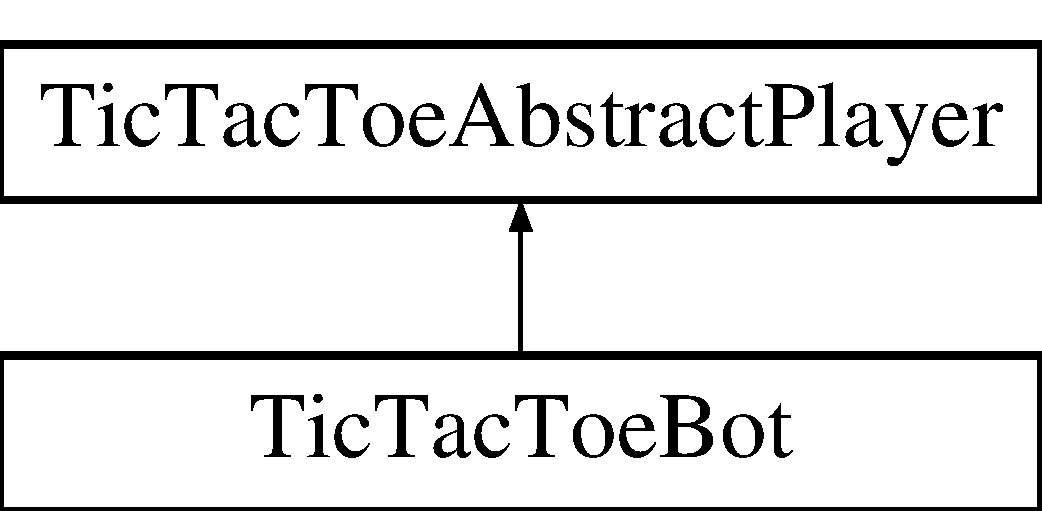
\includegraphics[height=2.000000cm]{class_tic_tac_toe_abstract_player}
\end{center}
\end{figure}
\subsection*{Public Member Functions}
\begin{DoxyCompactItemize}
\item 
\hyperlink{class_tic_tac_toe_abstract_player_a4a6df021e0dd3fa1e9a44fc7d9a4156a}{Tic\+Tac\+Toe\+Abstract\+Player} (size\+\_\+t size, \hyperlink{common__defs_8h_a9c8780378078e51e7c9041cbac392db9}{Player} player)
\item 
virtual void \hyperlink{class_tic_tac_toe_abstract_player_a0c307236b6413d44d2489f24ef85507a}{update} (const \hyperlink{common__defs_8h_a0dc5e1c0d1c3d4b1e210c805de5ca27b}{Board} \&board)
\item 
virtual \hyperlink{common__defs_8h_af9623b96ea87eb8f2d0fe97e45b0f79a}{Position} \hyperlink{class_tic_tac_toe_abstract_player_afccee4c01b399ecb12efc950474b6924}{move} ()=0
\item 
virtual void \hyperlink{class_tic_tac_toe_abstract_player_a4c36b375285f4d1511a11de121d0e5dc}{display} ()=0
\item 
virtual \hyperlink{class_tic_tac_toe_abstract_player_a5dbbe0fb30cd3acbae13d9a895b9bcd1}{$\sim$\+Tic\+Tac\+Toe\+Abstract\+Player} ()
\end{DoxyCompactItemize}
\subsection*{Protected Attributes}
\begin{DoxyCompactItemize}
\item 
size\+\_\+t \hyperlink{class_tic_tac_toe_abstract_player_a59c4f8555c74ce83ebabefc8199435e2}{size\+\_\+}
\item 
\hyperlink{common__defs_8h_a9c8780378078e51e7c9041cbac392db9}{Player} \hyperlink{class_tic_tac_toe_abstract_player_ace1857b73ea4e55c4ce6c00a3dcf12ec}{player\+\_\+}
\item 
\hyperlink{common__defs_8h_a0dc5e1c0d1c3d4b1e210c805de5ca27b}{Board} \hyperlink{class_tic_tac_toe_abstract_player_a5e35542f7b938692f77a0274849cad7f}{board\+\_\+}
\end{DoxyCompactItemize}


\subsection{Detailed Description}


Definition at line 5 of file tictactoeabstractplayer.\+h.



\subsection{Constructor \& Destructor Documentation}
\mbox{\Hypertarget{class_tic_tac_toe_abstract_player_a4a6df021e0dd3fa1e9a44fc7d9a4156a}\label{class_tic_tac_toe_abstract_player_a4a6df021e0dd3fa1e9a44fc7d9a4156a}} 
\index{Tic\+Tac\+Toe\+Abstract\+Player@{Tic\+Tac\+Toe\+Abstract\+Player}!Tic\+Tac\+Toe\+Abstract\+Player@{Tic\+Tac\+Toe\+Abstract\+Player}}
\index{Tic\+Tac\+Toe\+Abstract\+Player@{Tic\+Tac\+Toe\+Abstract\+Player}!Tic\+Tac\+Toe\+Abstract\+Player@{Tic\+Tac\+Toe\+Abstract\+Player}}
\subsubsection{\texorpdfstring{Tic\+Tac\+Toe\+Abstract\+Player()}{TicTacToeAbstractPlayer()}}
{\footnotesize\ttfamily Tic\+Tac\+Toe\+Abstract\+Player\+::\+Tic\+Tac\+Toe\+Abstract\+Player (\begin{DoxyParamCaption}\item[{size\+\_\+t}]{size,  }\item[{\hyperlink{common__defs_8h_a9c8780378078e51e7c9041cbac392db9}{Player}}]{player }\end{DoxyParamCaption})}



Definition at line 3 of file tictactoeabstractplayer.\+cpp.

\mbox{\Hypertarget{class_tic_tac_toe_abstract_player_a5dbbe0fb30cd3acbae13d9a895b9bcd1}\label{class_tic_tac_toe_abstract_player_a5dbbe0fb30cd3acbae13d9a895b9bcd1}} 
\index{Tic\+Tac\+Toe\+Abstract\+Player@{Tic\+Tac\+Toe\+Abstract\+Player}!````~Tic\+Tac\+Toe\+Abstract\+Player@{$\sim$\+Tic\+Tac\+Toe\+Abstract\+Player}}
\index{````~Tic\+Tac\+Toe\+Abstract\+Player@{$\sim$\+Tic\+Tac\+Toe\+Abstract\+Player}!Tic\+Tac\+Toe\+Abstract\+Player@{Tic\+Tac\+Toe\+Abstract\+Player}}
\subsubsection{\texorpdfstring{$\sim$\+Tic\+Tac\+Toe\+Abstract\+Player()}{~TicTacToeAbstractPlayer()}}
{\footnotesize\ttfamily Tic\+Tac\+Toe\+Abstract\+Player\+::$\sim$\+Tic\+Tac\+Toe\+Abstract\+Player (\begin{DoxyParamCaption}{ }\end{DoxyParamCaption})\hspace{0.3cm}{\ttfamily [virtual]}}



Definition at line 7 of file tictactoeabstractplayer.\+cpp.



\subsection{Member Function Documentation}
\mbox{\Hypertarget{class_tic_tac_toe_abstract_player_a4c36b375285f4d1511a11de121d0e5dc}\label{class_tic_tac_toe_abstract_player_a4c36b375285f4d1511a11de121d0e5dc}} 
\index{Tic\+Tac\+Toe\+Abstract\+Player@{Tic\+Tac\+Toe\+Abstract\+Player}!display@{display}}
\index{display@{display}!Tic\+Tac\+Toe\+Abstract\+Player@{Tic\+Tac\+Toe\+Abstract\+Player}}
\subsubsection{\texorpdfstring{display()}{display()}}
{\footnotesize\ttfamily virtual void Tic\+Tac\+Toe\+Abstract\+Player\+::display (\begin{DoxyParamCaption}{ }\end{DoxyParamCaption})\hspace{0.3cm}{\ttfamily [pure virtual]}}



Implemented in \hyperlink{class_tic_tac_toe_bot_a2af7f24506849f05ed37e9750b515c3d}{Tic\+Tac\+Toe\+Bot}.

\mbox{\Hypertarget{class_tic_tac_toe_abstract_player_afccee4c01b399ecb12efc950474b6924}\label{class_tic_tac_toe_abstract_player_afccee4c01b399ecb12efc950474b6924}} 
\index{Tic\+Tac\+Toe\+Abstract\+Player@{Tic\+Tac\+Toe\+Abstract\+Player}!move@{move}}
\index{move@{move}!Tic\+Tac\+Toe\+Abstract\+Player@{Tic\+Tac\+Toe\+Abstract\+Player}}
\subsubsection{\texorpdfstring{move()}{move()}}
{\footnotesize\ttfamily virtual \hyperlink{common__defs_8h_af9623b96ea87eb8f2d0fe97e45b0f79a}{Position} Tic\+Tac\+Toe\+Abstract\+Player\+::move (\begin{DoxyParamCaption}{ }\end{DoxyParamCaption})\hspace{0.3cm}{\ttfamily [pure virtual]}}



Implemented in \hyperlink{class_tic_tac_toe_bot_a66939785d51528036aab9cc37dd5fad5}{Tic\+Tac\+Toe\+Bot}.

\mbox{\Hypertarget{class_tic_tac_toe_abstract_player_a0c307236b6413d44d2489f24ef85507a}\label{class_tic_tac_toe_abstract_player_a0c307236b6413d44d2489f24ef85507a}} 
\index{Tic\+Tac\+Toe\+Abstract\+Player@{Tic\+Tac\+Toe\+Abstract\+Player}!update@{update}}
\index{update@{update}!Tic\+Tac\+Toe\+Abstract\+Player@{Tic\+Tac\+Toe\+Abstract\+Player}}
\subsubsection{\texorpdfstring{update()}{update()}}
{\footnotesize\ttfamily virtual void Tic\+Tac\+Toe\+Abstract\+Player\+::update (\begin{DoxyParamCaption}\item[{const \hyperlink{common__defs_8h_a0dc5e1c0d1c3d4b1e210c805de5ca27b}{Board} \&}]{board }\end{DoxyParamCaption})\hspace{0.3cm}{\ttfamily [inline]}, {\ttfamily [virtual]}}



Definition at line 14 of file tictactoeabstractplayer.\+h.



\subsection{Member Data Documentation}
\mbox{\Hypertarget{class_tic_tac_toe_abstract_player_a5e35542f7b938692f77a0274849cad7f}\label{class_tic_tac_toe_abstract_player_a5e35542f7b938692f77a0274849cad7f}} 
\index{Tic\+Tac\+Toe\+Abstract\+Player@{Tic\+Tac\+Toe\+Abstract\+Player}!board\+\_\+@{board\+\_\+}}
\index{board\+\_\+@{board\+\_\+}!Tic\+Tac\+Toe\+Abstract\+Player@{Tic\+Tac\+Toe\+Abstract\+Player}}
\subsubsection{\texorpdfstring{board\+\_\+}{board\_}}
{\footnotesize\ttfamily \hyperlink{common__defs_8h_a0dc5e1c0d1c3d4b1e210c805de5ca27b}{Board} Tic\+Tac\+Toe\+Abstract\+Player\+::board\+\_\+\hspace{0.3cm}{\ttfamily [protected]}}



Definition at line 10 of file tictactoeabstractplayer.\+h.

\mbox{\Hypertarget{class_tic_tac_toe_abstract_player_ace1857b73ea4e55c4ce6c00a3dcf12ec}\label{class_tic_tac_toe_abstract_player_ace1857b73ea4e55c4ce6c00a3dcf12ec}} 
\index{Tic\+Tac\+Toe\+Abstract\+Player@{Tic\+Tac\+Toe\+Abstract\+Player}!player\+\_\+@{player\+\_\+}}
\index{player\+\_\+@{player\+\_\+}!Tic\+Tac\+Toe\+Abstract\+Player@{Tic\+Tac\+Toe\+Abstract\+Player}}
\subsubsection{\texorpdfstring{player\+\_\+}{player\_}}
{\footnotesize\ttfamily \hyperlink{common__defs_8h_a9c8780378078e51e7c9041cbac392db9}{Player} Tic\+Tac\+Toe\+Abstract\+Player\+::player\+\_\+\hspace{0.3cm}{\ttfamily [protected]}}



Definition at line 9 of file tictactoeabstractplayer.\+h.

\mbox{\Hypertarget{class_tic_tac_toe_abstract_player_a59c4f8555c74ce83ebabefc8199435e2}\label{class_tic_tac_toe_abstract_player_a59c4f8555c74ce83ebabefc8199435e2}} 
\index{Tic\+Tac\+Toe\+Abstract\+Player@{Tic\+Tac\+Toe\+Abstract\+Player}!size\+\_\+@{size\+\_\+}}
\index{size\+\_\+@{size\+\_\+}!Tic\+Tac\+Toe\+Abstract\+Player@{Tic\+Tac\+Toe\+Abstract\+Player}}
\subsubsection{\texorpdfstring{size\+\_\+}{size\_}}
{\footnotesize\ttfamily size\+\_\+t Tic\+Tac\+Toe\+Abstract\+Player\+::size\+\_\+\hspace{0.3cm}{\ttfamily [protected]}}



Definition at line 8 of file tictactoeabstractplayer.\+h.



The documentation for this class was generated from the following files\+:\begin{DoxyCompactItemize}
\item 
\hyperlink{tictactoeabstractplayer_8h}{tictactoeabstractplayer.\+h}\item 
\hyperlink{tictactoeabstractplayer_8cpp}{tictactoeabstractplayer.\+cpp}\end{DoxyCompactItemize}

\hypertarget{class_tic_tac_toe_bot}{}\section{Tic\+Tac\+Toe\+Bot Class Reference}
\label{class_tic_tac_toe_bot}\index{Tic\+Tac\+Toe\+Bot@{Tic\+Tac\+Toe\+Bot}}


{\ttfamily \#include $<$tictactoebot.\+h$>$}

Inheritance diagram for Tic\+Tac\+Toe\+Bot\+:\begin{figure}[H]
\begin{center}
\leavevmode
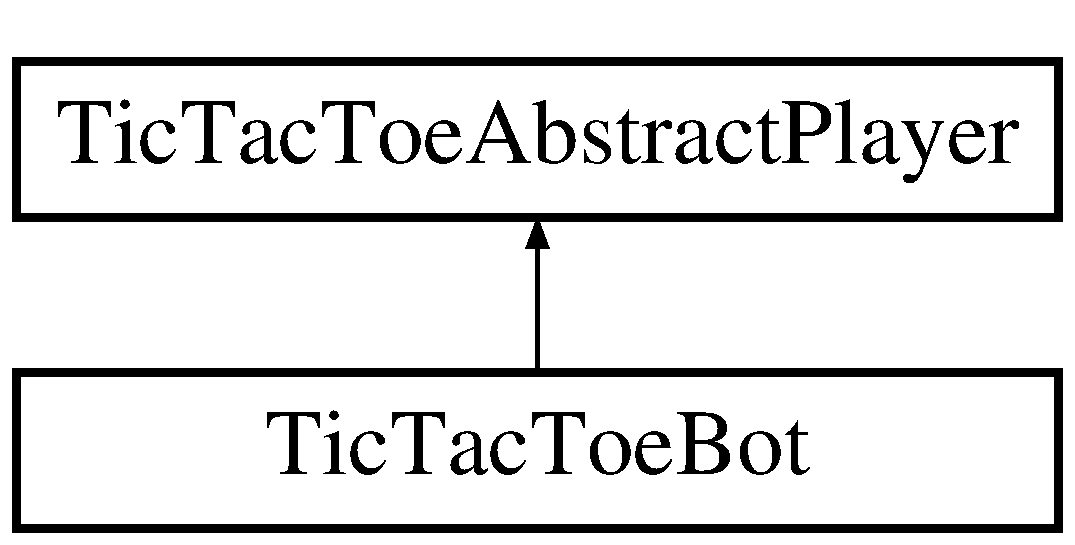
\includegraphics[height=2.000000cm]{class_tic_tac_toe_bot}
\end{center}
\end{figure}
\subsection*{Public Member Functions}
\begin{DoxyCompactItemize}
\item 
\hyperlink{class_tic_tac_toe_bot_acad176967b40f0b38444cc56e90b07c3}{Tic\+Tac\+Toe\+Bot} (size\+\_\+t size, \hyperlink{common__defs_8h_a9c8780378078e51e7c9041cbac392db9}{Player} player)
\item 
\hyperlink{common__defs_8h_af9623b96ea87eb8f2d0fe97e45b0f79a}{Position} \hyperlink{class_tic_tac_toe_bot_a66939785d51528036aab9cc37dd5fad5}{move} ()
\item 
void \hyperlink{class_tic_tac_toe_bot_a2af7f24506849f05ed37e9750b515c3d}{display} ()
\end{DoxyCompactItemize}
\subsection*{Additional Inherited Members}


\subsection{Detailed Description}


Definition at line 9 of file tictactoebot.\+h.



\subsection{Constructor \& Destructor Documentation}
\mbox{\Hypertarget{class_tic_tac_toe_bot_acad176967b40f0b38444cc56e90b07c3}\label{class_tic_tac_toe_bot_acad176967b40f0b38444cc56e90b07c3}} 
\index{Tic\+Tac\+Toe\+Bot@{Tic\+Tac\+Toe\+Bot}!Tic\+Tac\+Toe\+Bot@{Tic\+Tac\+Toe\+Bot}}
\index{Tic\+Tac\+Toe\+Bot@{Tic\+Tac\+Toe\+Bot}!Tic\+Tac\+Toe\+Bot@{Tic\+Tac\+Toe\+Bot}}
\subsubsection{\texorpdfstring{Tic\+Tac\+Toe\+Bot()}{TicTacToeBot()}}
{\footnotesize\ttfamily Tic\+Tac\+Toe\+Bot\+::\+Tic\+Tac\+Toe\+Bot (\begin{DoxyParamCaption}\item[{size\+\_\+t}]{size,  }\item[{\hyperlink{common__defs_8h_a9c8780378078e51e7c9041cbac392db9}{Player}}]{player }\end{DoxyParamCaption})\hspace{0.3cm}{\ttfamily [inline]}}



Definition at line 18 of file tictactoebot.\+h.



\subsection{Member Function Documentation}
\mbox{\Hypertarget{class_tic_tac_toe_bot_a2af7f24506849f05ed37e9750b515c3d}\label{class_tic_tac_toe_bot_a2af7f24506849f05ed37e9750b515c3d}} 
\index{Tic\+Tac\+Toe\+Bot@{Tic\+Tac\+Toe\+Bot}!display@{display}}
\index{display@{display}!Tic\+Tac\+Toe\+Bot@{Tic\+Tac\+Toe\+Bot}}
\subsubsection{\texorpdfstring{display()}{display()}}
{\footnotesize\ttfamily void Tic\+Tac\+Toe\+Bot\+::display (\begin{DoxyParamCaption}{ }\end{DoxyParamCaption})\hspace{0.3cm}{\ttfamily [virtual]}}



Implements \hyperlink{class_tic_tac_toe_abstract_player_a4c36b375285f4d1511a11de121d0e5dc}{Tic\+Tac\+Toe\+Abstract\+Player}.



Definition at line 13 of file tictactoebot.\+cpp.

\mbox{\Hypertarget{class_tic_tac_toe_bot_a66939785d51528036aab9cc37dd5fad5}\label{class_tic_tac_toe_bot_a66939785d51528036aab9cc37dd5fad5}} 
\index{Tic\+Tac\+Toe\+Bot@{Tic\+Tac\+Toe\+Bot}!move@{move}}
\index{move@{move}!Tic\+Tac\+Toe\+Bot@{Tic\+Tac\+Toe\+Bot}}
\subsubsection{\texorpdfstring{move()}{move()}}
{\footnotesize\ttfamily \hyperlink{common__defs_8h_af9623b96ea87eb8f2d0fe97e45b0f79a}{Position} Tic\+Tac\+Toe\+Bot\+::move (\begin{DoxyParamCaption}{ }\end{DoxyParamCaption})\hspace{0.3cm}{\ttfamily [virtual]}}



Implements \hyperlink{class_tic_tac_toe_abstract_player_afccee4c01b399ecb12efc950474b6924}{Tic\+Tac\+Toe\+Abstract\+Player}.



Definition at line 3 of file tictactoebot.\+cpp.



The documentation for this class was generated from the following files\+:\begin{DoxyCompactItemize}
\item 
\hyperlink{tictactoebot_8h}{tictactoebot.\+h}\item 
\hyperlink{tictactoebot_8cpp}{tictactoebot.\+cpp}\end{DoxyCompactItemize}

\chapter{File Documentation}
\hypertarget{common__defs_8h}{}\section{common\+\_\+defs.\+h File Reference}
\label{common__defs_8h}\index{common\+\_\+defs.\+h@{common\+\_\+defs.\+h}}
{\ttfamily \#include $<$vector$>$}\newline
\subsection*{Typedefs}
\begin{DoxyCompactItemize}
\item 
using \hyperlink{common__defs_8h_a0dc5e1c0d1c3d4b1e210c805de5ca27b}{Board} = std\+::vector$<$ std\+::vector$<$ \hyperlink{common__defs_8h_a9c8780378078e51e7c9041cbac392db9}{Player} $>$ $>$
\item 
using \hyperlink{common__defs_8h_af9623b96ea87eb8f2d0fe97e45b0f79a}{Position} = std\+::pair$<$ size\+\_\+t, size\+\_\+t $>$
\end{DoxyCompactItemize}
\subsection*{Enumerations}
\begin{DoxyCompactItemize}
\item 
enum \hyperlink{common__defs_8h_a9c8780378078e51e7c9041cbac392db9}{Player} \{ \hyperlink{common__defs_8h_a9c8780378078e51e7c9041cbac392db9a37a6259cc0c1dae299a7866489dff0bd}{Player\+::null} = 0, 
\hyperlink{common__defs_8h_a9c8780378078e51e7c9041cbac392db9a22aadb26447d87b550b155a4d764fad0}{Player\+::cross}, 
\hyperlink{common__defs_8h_a9c8780378078e51e7c9041cbac392db9a9b6ddeba5b33e577c07c35d8505c6072}{Player\+::circle}
 \}
\item 
enum \hyperlink{common__defs_8h_a67a0db04d321a74b7e7fcfd3f1a3f70b}{Status} \{ \hyperlink{common__defs_8h_a67a0db04d321a74b7e7fcfd3f1a3f70ba3734a903022249b3010be1897042568e}{Status\+::move} = 0, 
\hyperlink{common__defs_8h_a67a0db04d321a74b7e7fcfd3f1a3f70ba0b08bd98d279b88859b628cd8c061ae0}{Status\+::win}, 
\hyperlink{common__defs_8h_a67a0db04d321a74b7e7fcfd3f1a3f70ba817491bc777731f0f0c6e485f28e4d86}{Status\+::draw}
 \}
\end{DoxyCompactItemize}


\subsection{Typedef Documentation}
\mbox{\Hypertarget{common__defs_8h_a0dc5e1c0d1c3d4b1e210c805de5ca27b}\label{common__defs_8h_a0dc5e1c0d1c3d4b1e210c805de5ca27b}} 
\index{common\+\_\+defs.\+h@{common\+\_\+defs.\+h}!Board@{Board}}
\index{Board@{Board}!common\+\_\+defs.\+h@{common\+\_\+defs.\+h}}
\subsubsection{\texorpdfstring{Board}{Board}}
{\footnotesize\ttfamily using \hyperlink{common__defs_8h_a0dc5e1c0d1c3d4b1e210c805de5ca27b}{Board} =  std\+::vector$<$std\+::vector$<$\hyperlink{common__defs_8h_a9c8780378078e51e7c9041cbac392db9}{Player}$>$ $>$}



Definition at line 6 of file common\+\_\+defs.\+h.

\mbox{\Hypertarget{common__defs_8h_af9623b96ea87eb8f2d0fe97e45b0f79a}\label{common__defs_8h_af9623b96ea87eb8f2d0fe97e45b0f79a}} 
\index{common\+\_\+defs.\+h@{common\+\_\+defs.\+h}!Position@{Position}}
\index{Position@{Position}!common\+\_\+defs.\+h@{common\+\_\+defs.\+h}}
\subsubsection{\texorpdfstring{Position}{Position}}
{\footnotesize\ttfamily using \hyperlink{common__defs_8h_af9623b96ea87eb8f2d0fe97e45b0f79a}{Position} =  std\+::pair$<$size\+\_\+t, size\+\_\+t$>$}



Definition at line 7 of file common\+\_\+defs.\+h.



\subsection{Enumeration Type Documentation}
\mbox{\Hypertarget{common__defs_8h_a9c8780378078e51e7c9041cbac392db9}\label{common__defs_8h_a9c8780378078e51e7c9041cbac392db9}} 
\index{common\+\_\+defs.\+h@{common\+\_\+defs.\+h}!Player@{Player}}
\index{Player@{Player}!common\+\_\+defs.\+h@{common\+\_\+defs.\+h}}
\subsubsection{\texorpdfstring{Player}{Player}}
{\footnotesize\ttfamily enum \hyperlink{common__defs_8h_a9c8780378078e51e7c9041cbac392db9}{Player}\hspace{0.3cm}{\ttfamily [strong]}}

\begin{DoxyEnumFields}{Enumerator}
\raisebox{\heightof{T}}[0pt][0pt]{\index{null@{null}!common\+\_\+defs.\+h@{common\+\_\+defs.\+h}}\index{common\+\_\+defs.\+h@{common\+\_\+defs.\+h}!null@{null}}}\mbox{\Hypertarget{common__defs_8h_a9c8780378078e51e7c9041cbac392db9a37a6259cc0c1dae299a7866489dff0bd}\label{common__defs_8h_a9c8780378078e51e7c9041cbac392db9a37a6259cc0c1dae299a7866489dff0bd}} 
null&\\
\hline

\raisebox{\heightof{T}}[0pt][0pt]{\index{cross@{cross}!common\+\_\+defs.\+h@{common\+\_\+defs.\+h}}\index{common\+\_\+defs.\+h@{common\+\_\+defs.\+h}!cross@{cross}}}\mbox{\Hypertarget{common__defs_8h_a9c8780378078e51e7c9041cbac392db9a22aadb26447d87b550b155a4d764fad0}\label{common__defs_8h_a9c8780378078e51e7c9041cbac392db9a22aadb26447d87b550b155a4d764fad0}} 
cross&\\
\hline

\raisebox{\heightof{T}}[0pt][0pt]{\index{circle@{circle}!common\+\_\+defs.\+h@{common\+\_\+defs.\+h}}\index{common\+\_\+defs.\+h@{common\+\_\+defs.\+h}!circle@{circle}}}\mbox{\Hypertarget{common__defs_8h_a9c8780378078e51e7c9041cbac392db9a9b6ddeba5b33e577c07c35d8505c6072}\label{common__defs_8h_a9c8780378078e51e7c9041cbac392db9a9b6ddeba5b33e577c07c35d8505c6072}} 
circle&\\
\hline

\end{DoxyEnumFields}


Definition at line 4 of file common\+\_\+defs.\+h.

\mbox{\Hypertarget{common__defs_8h_a67a0db04d321a74b7e7fcfd3f1a3f70b}\label{common__defs_8h_a67a0db04d321a74b7e7fcfd3f1a3f70b}} 
\index{common\+\_\+defs.\+h@{common\+\_\+defs.\+h}!Status@{Status}}
\index{Status@{Status}!common\+\_\+defs.\+h@{common\+\_\+defs.\+h}}
\subsubsection{\texorpdfstring{Status}{Status}}
{\footnotesize\ttfamily enum \hyperlink{common__defs_8h_a67a0db04d321a74b7e7fcfd3f1a3f70b}{Status}\hspace{0.3cm}{\ttfamily [strong]}}

\begin{DoxyEnumFields}{Enumerator}
\raisebox{\heightof{T}}[0pt][0pt]{\index{move@{move}!common\+\_\+defs.\+h@{common\+\_\+defs.\+h}}\index{common\+\_\+defs.\+h@{common\+\_\+defs.\+h}!move@{move}}}\mbox{\Hypertarget{common__defs_8h_a67a0db04d321a74b7e7fcfd3f1a3f70ba3734a903022249b3010be1897042568e}\label{common__defs_8h_a67a0db04d321a74b7e7fcfd3f1a3f70ba3734a903022249b3010be1897042568e}} 
move&\\
\hline

\raisebox{\heightof{T}}[0pt][0pt]{\index{win@{win}!common\+\_\+defs.\+h@{common\+\_\+defs.\+h}}\index{common\+\_\+defs.\+h@{common\+\_\+defs.\+h}!win@{win}}}\mbox{\Hypertarget{common__defs_8h_a67a0db04d321a74b7e7fcfd3f1a3f70ba0b08bd98d279b88859b628cd8c061ae0}\label{common__defs_8h_a67a0db04d321a74b7e7fcfd3f1a3f70ba0b08bd98d279b88859b628cd8c061ae0}} 
win&\\
\hline

\raisebox{\heightof{T}}[0pt][0pt]{\index{draw@{draw}!common\+\_\+defs.\+h@{common\+\_\+defs.\+h}}\index{common\+\_\+defs.\+h@{common\+\_\+defs.\+h}!draw@{draw}}}\mbox{\Hypertarget{common__defs_8h_a67a0db04d321a74b7e7fcfd3f1a3f70ba817491bc777731f0f0c6e485f28e4d86}\label{common__defs_8h_a67a0db04d321a74b7e7fcfd3f1a3f70ba817491bc777731f0f0c6e485f28e4d86}} 
draw&\\
\hline

\end{DoxyEnumFields}


Definition at line 5 of file common\+\_\+defs.\+h.


\hypertarget{main_8cpp}{}\section{main.\+cpp File Reference}
\label{main_8cpp}\index{main.\+cpp@{main.\+cpp}}
{\ttfamily \#include $<$iostream$>$}\newline
{\ttfamily \#include $<$tictactoe.\+h$>$}\newline
{\ttfamily \#include $<$tictactoebot.\+h$>$}\newline
\subsection*{Functions}
\begin{DoxyCompactItemize}
\item 
int \hyperlink{main_8cpp_ae66f6b31b5ad750f1fe042a706a4e3d4}{main} ()
\end{DoxyCompactItemize}


\subsection{Function Documentation}
\mbox{\Hypertarget{main_8cpp_ae66f6b31b5ad750f1fe042a706a4e3d4}\label{main_8cpp_ae66f6b31b5ad750f1fe042a706a4e3d4}} 
\index{main.\+cpp@{main.\+cpp}!main@{main}}
\index{main@{main}!main.\+cpp@{main.\+cpp}}
\subsubsection{\texorpdfstring{main()}{main()}}
{\footnotesize\ttfamily int main (\begin{DoxyParamCaption}{ }\end{DoxyParamCaption})}



Definition at line 6 of file main.\+cpp.


\hypertarget{tictactoe_8cpp}{}\section{tictactoe.\+cpp File Reference}
\label{tictactoe_8cpp}\index{tictactoe.\+cpp@{tictactoe.\+cpp}}
{\ttfamily \#include \char`\"{}tictactoe.\+h\char`\"{}}\newline

\hypertarget{tictactoe_8h}{}\section{tictactoe.\+h File Reference}
\label{tictactoe_8h}\index{tictactoe.\+h@{tictactoe.\+h}}
{\ttfamily \#include \char`\"{}common\+\_\+defs.\+h\char`\"{}}\newline
{\ttfamily \#include $<$algorithm$>$}\newline
{\ttfamily \#include $<$iostream$>$}\newline
{\ttfamily \#include $<$vector$>$}\newline
\subsection*{Classes}
\begin{DoxyCompactItemize}
\item 
class \hyperlink{class_tic_tac_toe}{Tic\+Tac\+Toe}
\end{DoxyCompactItemize}

\hypertarget{tictactoeabstractplayer_8cpp}{}\section{tictactoeabstractplayer.\+cpp File Reference}
\label{tictactoeabstractplayer_8cpp}\index{tictactoeabstractplayer.\+cpp@{tictactoeabstractplayer.\+cpp}}
{\ttfamily \#include \char`\"{}tictactoeabstractplayer.\+h\char`\"{}}\newline

\hypertarget{tictactoeabstractplayer_8h}{}\section{tictactoeabstractplayer.\+h File Reference}
\label{tictactoeabstractplayer_8h}\index{tictactoeabstractplayer.\+h@{tictactoeabstractplayer.\+h}}
{\ttfamily \#include \char`\"{}common\+\_\+defs.\+h\char`\"{}}\newline
{\ttfamily \#include $<$vector$>$}\newline
\subsection*{Classes}
\begin{DoxyCompactItemize}
\item 
class \hyperlink{class_tic_tac_toe_abstract_player}{Tic\+Tac\+Toe\+Abstract\+Player}
\end{DoxyCompactItemize}

\hypertarget{tictactoebot_8cpp}{}\section{tictactoebot.\+cpp File Reference}
\label{tictactoebot_8cpp}\index{tictactoebot.\+cpp@{tictactoebot.\+cpp}}
{\ttfamily \#include \char`\"{}tictactoebot.\+h\char`\"{}}\newline

\hypertarget{tictactoebot_8h}{}\section{tictactoebot.\+h File Reference}
\label{tictactoebot_8h}\index{tictactoebot.\+h@{tictactoebot.\+h}}
{\ttfamily \#include \char`\"{}common\+\_\+defs.\+h\char`\"{}}\newline
{\ttfamily \#include \char`\"{}tictactoe.\+h\char`\"{}}\newline
{\ttfamily \#include \char`\"{}tictactoeabstractplayer.\+h\char`\"{}}\newline
{\ttfamily \#include $<$list$>$}\newline
\subsection*{Classes}
\begin{DoxyCompactItemize}
\item 
class \hyperlink{class_tic_tac_toe_bot}{Tic\+Tac\+Toe\+Bot}
\end{DoxyCompactItemize}

%--- End generated contents ---

% Index
\backmatter
\newpage
\phantomsection
\clearemptydoublepage
\addcontentsline{toc}{chapter}{Index}
\printindex

\end{document}
